\chapter{Auswertung der Messdaten und Diskussion}

\section{Photolumineszenz (PL) und Direktionalität bei konstanter Temperatur}~\label{sec:PL_u_Direktionalitaet}
%Im folgenden Abschnitt wird die beobachtete Photolumineszenz und die Direktionalität
%bei einer Temperatur von $\SI{4}{\kelvin}$ diskutiert.
Die gemessene Photolumineszenz der Probe(\ref{fig:probe})
ist in Abbildung~\ref{fig:photo} zu sehen. Die Probentemperatur hat $T = \SI{4}{\kelvin}$ betragen.
Das Maximum der PL liegt bei $\SI{737}{\nano\meter}$ und ist als Gaußsche Glockenfunktion in Abbildung~\ref{fig:max}
zu sehen.
Die Wellenlänge im Maximum entspricht einer Energie von $\SI{1,68}{\eV}$.
\begin{figure}
    \centering
    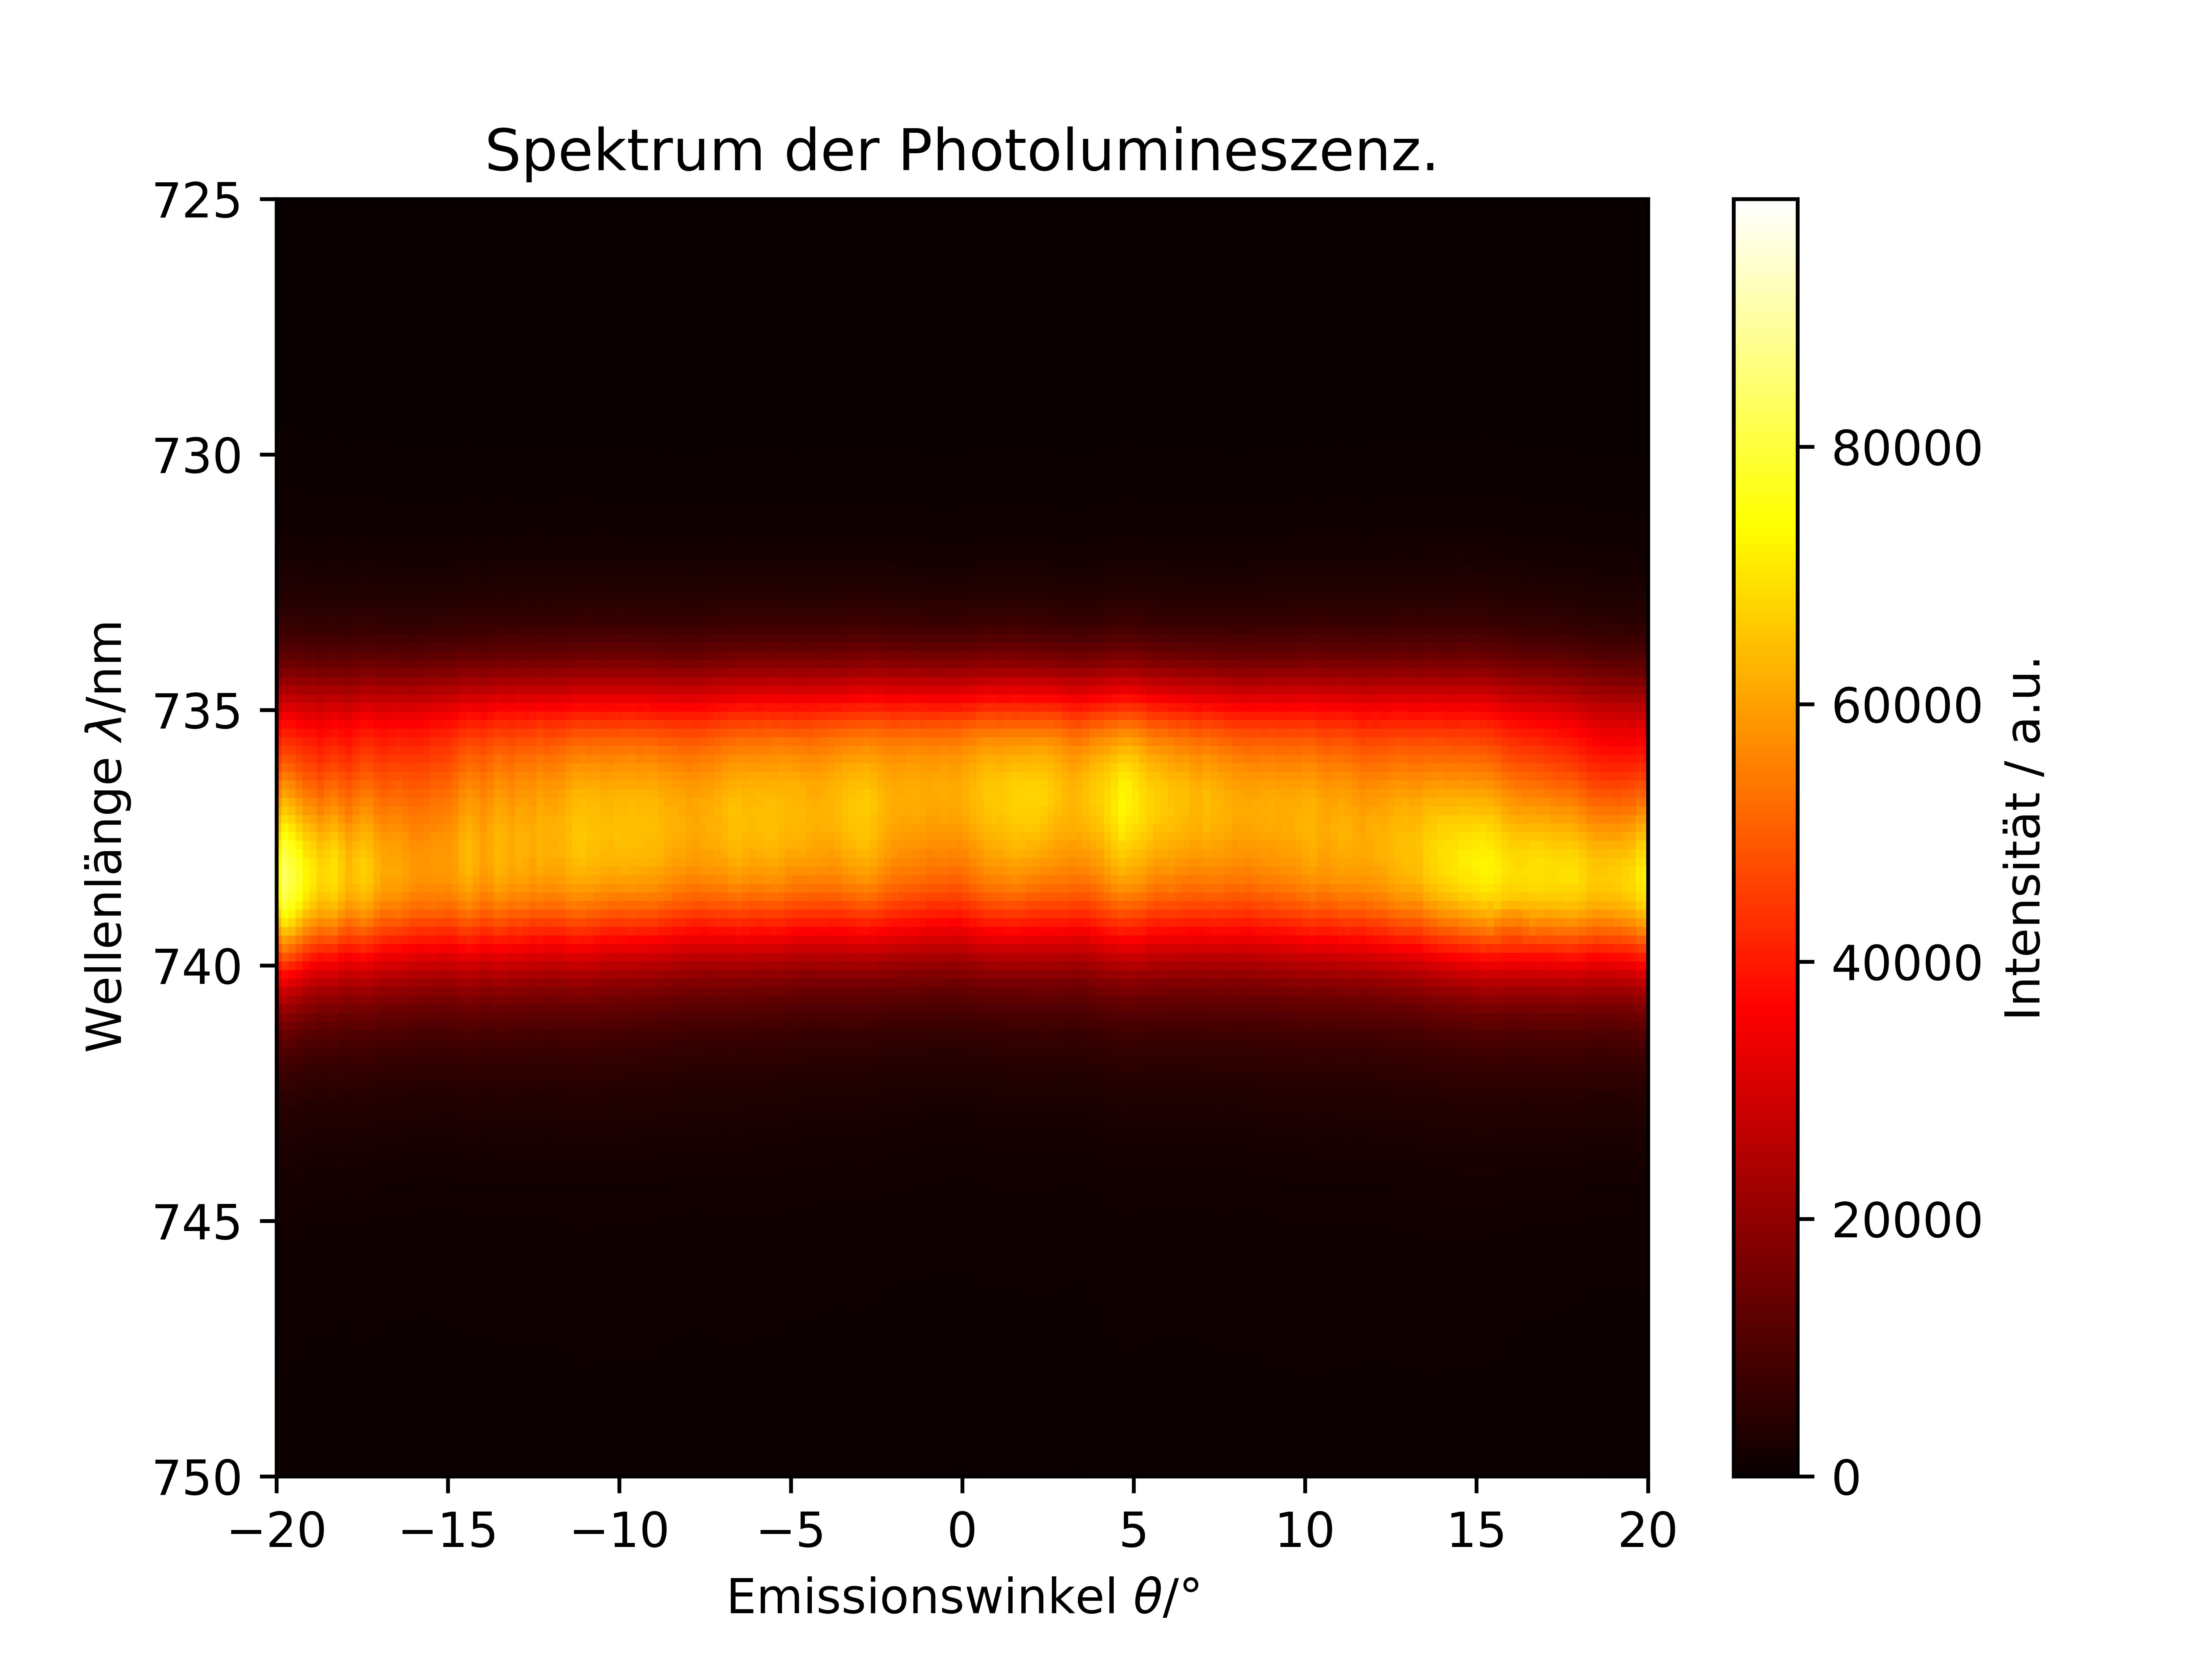
\includegraphics[scale=0.7]{./Plots/colormap__intensity_photolumineszenz_022818A 250nm 4K 2020-07-14.png}
    \caption{Gemessene PL bei einer Temperatur von $\SI{4}{\kelvin}$. 
    Das Maximus ist bei $\SI{737}{\nano\meter}$. 
    Je heller die Bereiche desto mehr Intensität ist an der Stelle gemessen worden.}
    \label{fig:photo}
\end{figure}
\FloatBarrier
%%%%%%%%%%%%%%%%%%%%%%%%%%%%%%%%%%%%%%%%%%%%%%%%%%%%%%%%%%%%%%%%%%%%%%%%%%%%%%%%%%%%%%%%%%%%%%%%%%%
\begin{figure}
    %\centering
    \begin{subfigure}{0.5\textwidth}
       %\centering
        \includegraphics[scale=0.45]{./Plots/max_value_Pl.pdf}
        \caption{Darstellung des Intensitätsmaximums, der im Experiment gemessenen Photolumineszenz, der Probe.}
        \label{fig:max}
    \end{subfigure}
    \begin{subfigure}{0.5\textwidth}
        %\centering
        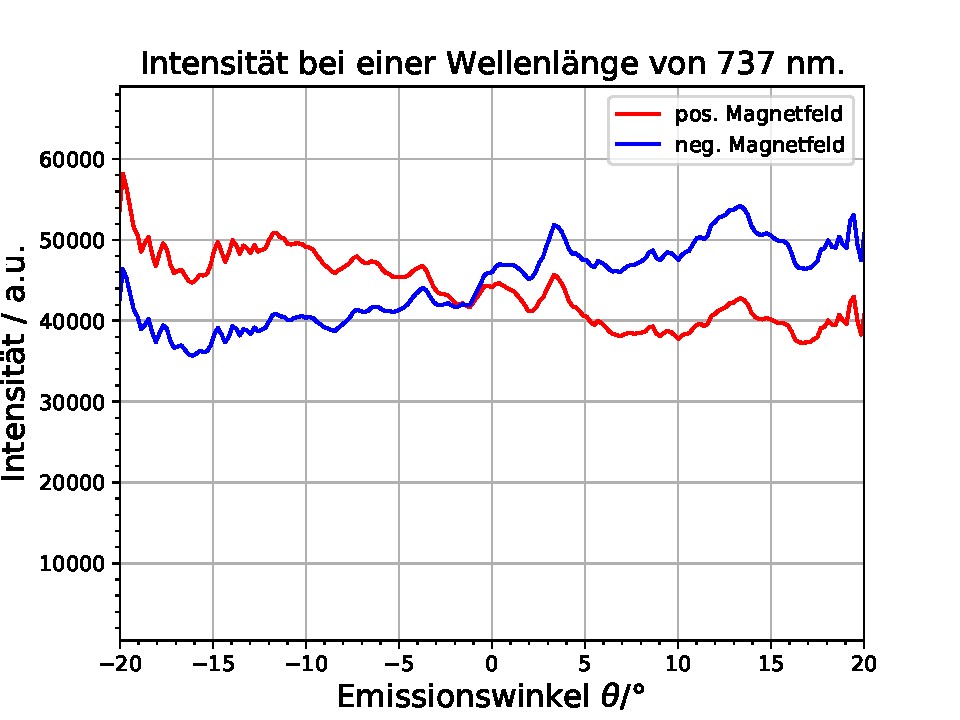
\includegraphics[scale=0.45]{./Plots/positive_and_negative_intensity_at_specific_wavelength_737_nm_022818A 250nm 4K 2020-07-14.pdf}
        \caption{Darstellung des Intensitätsverlaufs der Probe beim Wechsel von positiven zu negativen Magnetfeld.}
        \label{fig:i_pn}
    \end{subfigure}
    \caption{In der linken Abbildung ist das Maximum der PL der verwendeten Probe zu sehen,
                in der rechten die unterschiedlichen Intensitäten bei positiven und negativen Magnetfeld. }
    \label{fig:rho}
\end{figure}
\FloatBarrier
%%%%%%%%%%%%%%%%%%%%%%%%%%%%%%%%%%%%%%%%%%%%%%%%%%%%%%%%%%%%%%%%%%%%%%%%%%%%%%%%%%%%%%%%%%%%%%%%%%%
%\begin{figure}
%    \centering
%    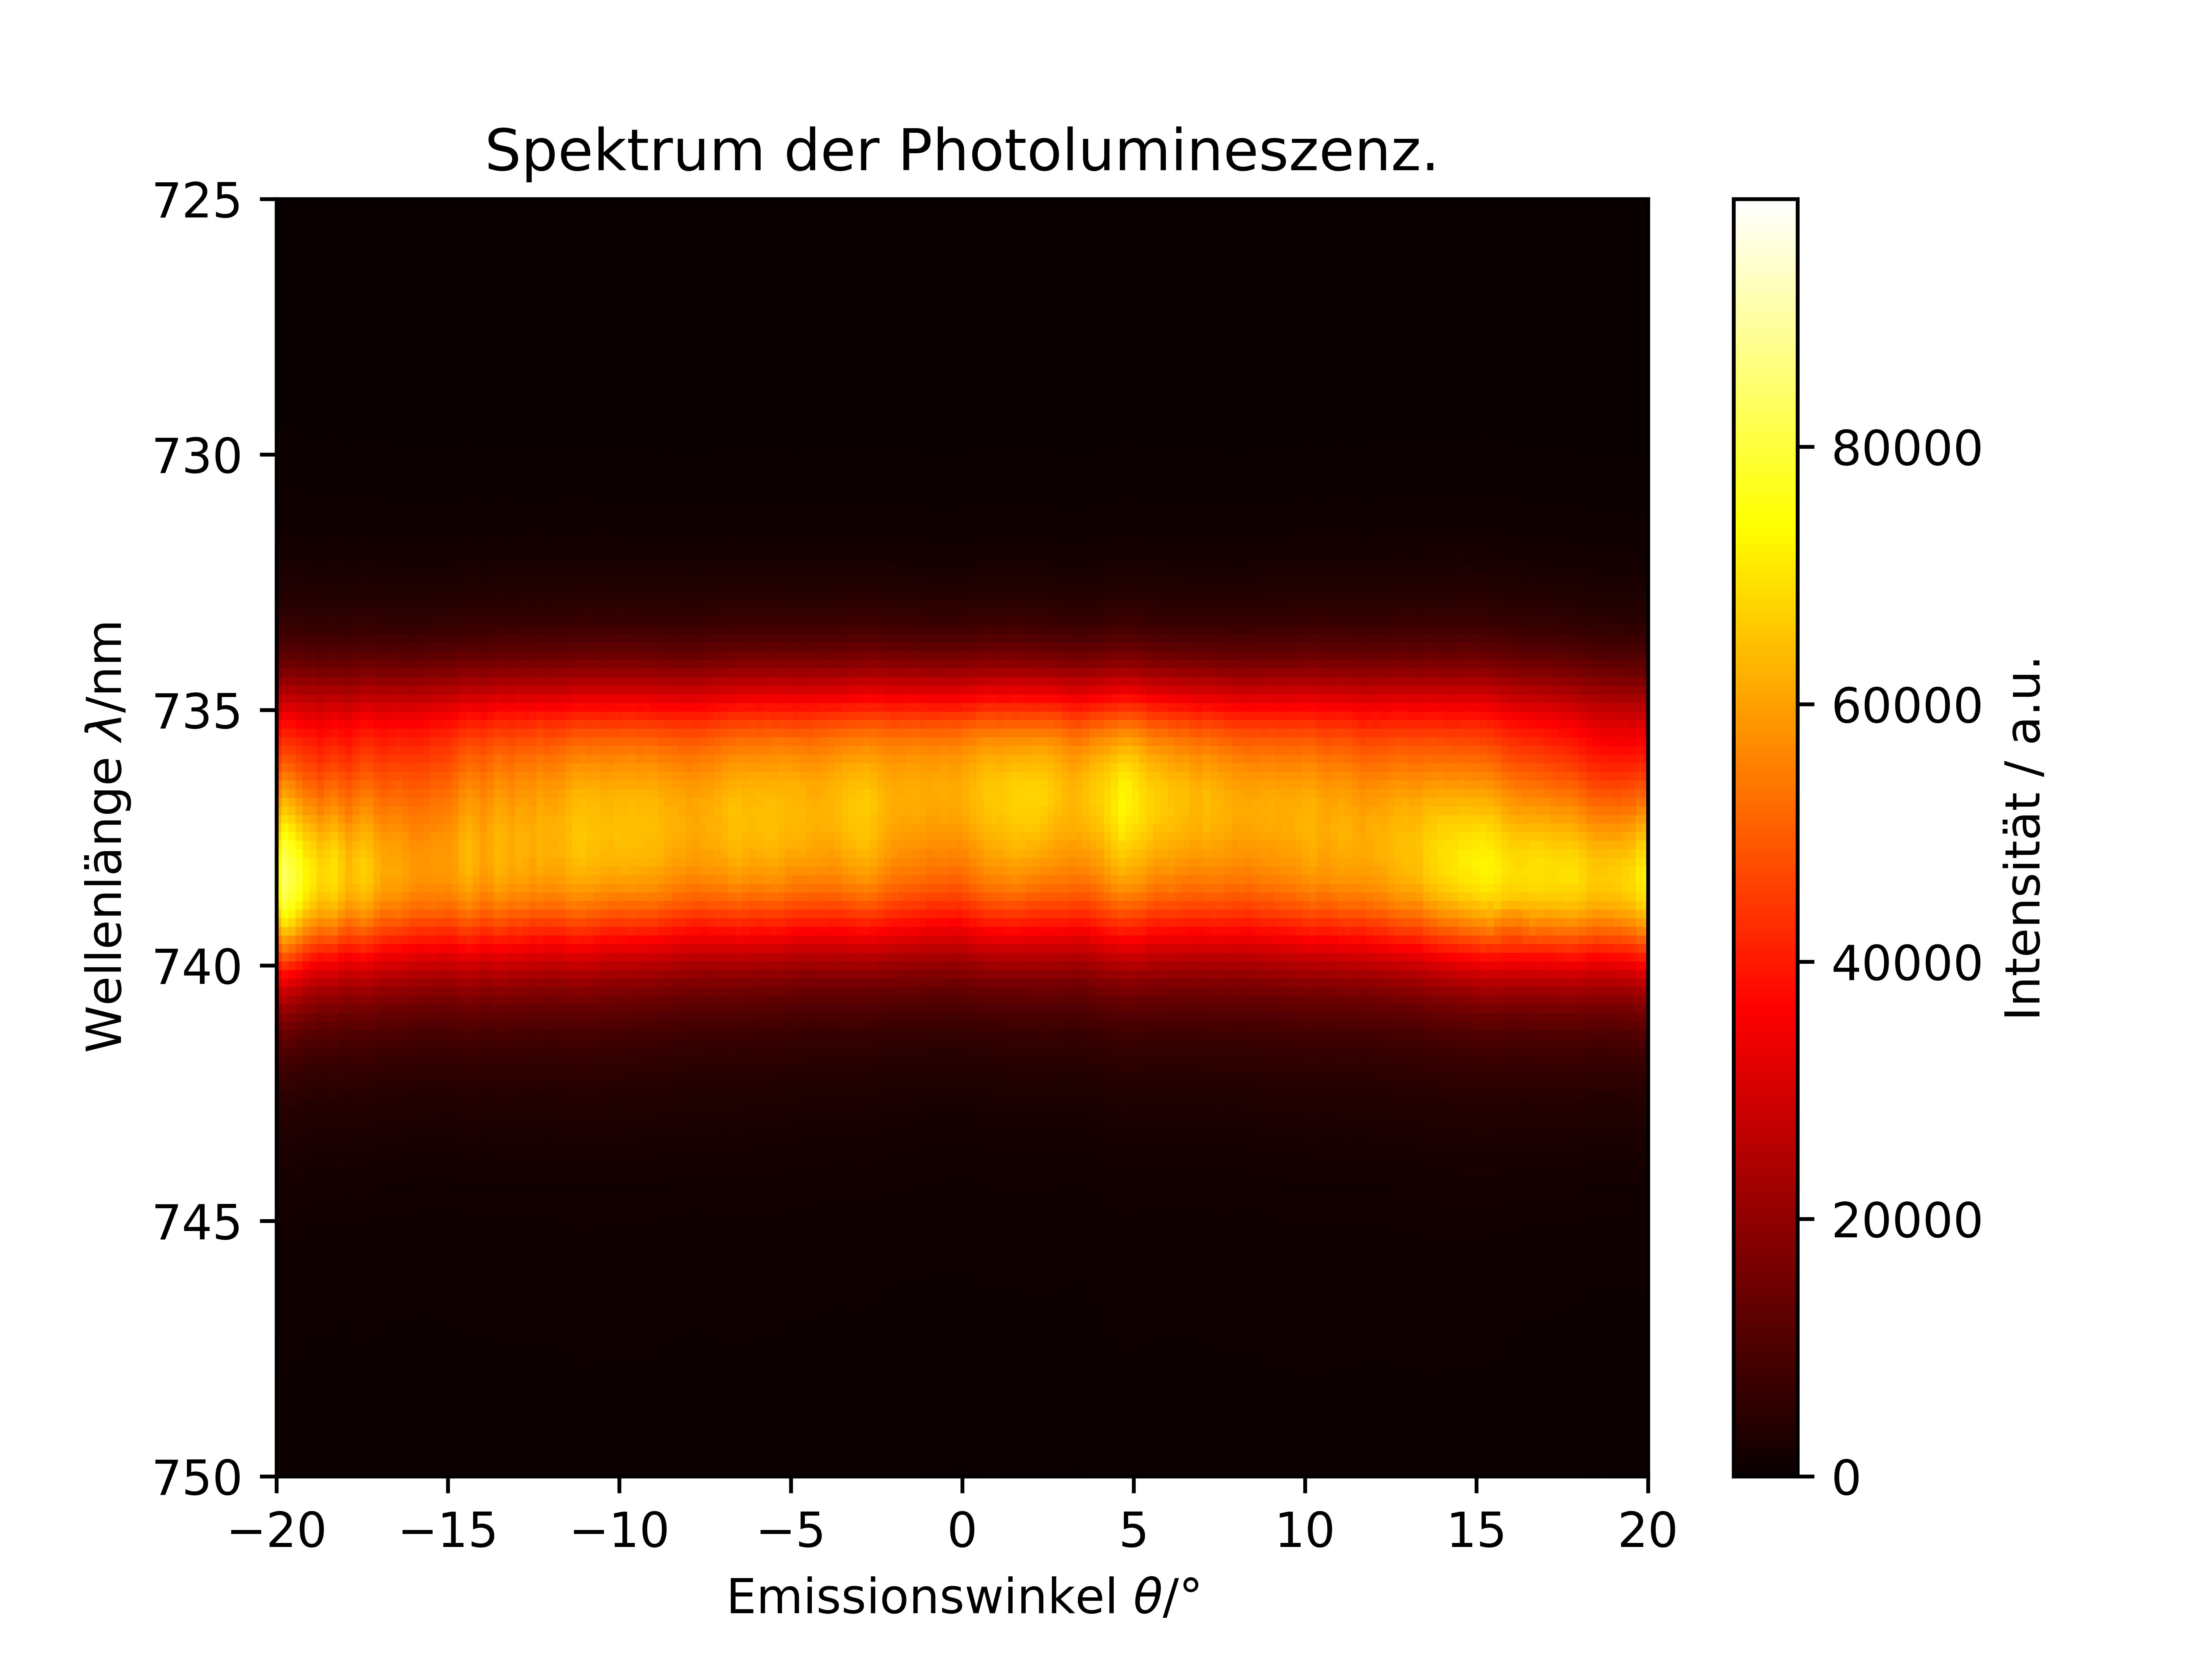
\includegraphics[scale=0.6]{./Plots/colormap__intensity_photolumineszenz_022818A 250nm 4K 2020-07-14.png}
%    \caption{Gemessene PL bei einer Temperatur von $\SI{4}{\kelvin}$. 
%    Das Maximus ist bei $\SI{737}{\nano\meter}$. 
%    Je heller die Bereiche desto mehr Intensität ist an der Stelle gemessen worden.}
%    \label{fig:photo}
%\end{figure}
%\FloatBarrier

Die von der Probe emittierte Wellenlänge liegt im sichtbaren Bereich und war real im Experiment als rotes Licht zu erkennen.
Der Winkelbereich wird bei Winkelabhängigen Messungen auf $\theta = \pm \SI{20}{\degree}$ 
eingeschränkt um störende Randeffekte/Artefakte zu vermeiden. 
Der Tatsächlich auflösbare Winkelbereich, aufgrund der numerischen Apertur, liegt bei $\theta = \pm \SI{24}{\degree}$ 
(vgl. Abschnitt~\ref{sec:Beschreibung des Versuchsaufbaus}).
Die abgebildete PL ist durch die Summation aller Einzelmessungen 
bei positiven und negativen Magnetfeld entstanden. 
Wie in Abbildung~\ref{fig:photo} zu erkennen, ist die Intensität homogen über den Winkelbereich verteilt.
Daraus lässt sich schließen, dass es bei dem Effekt keine bevorzugte Polung des Magnetfelds
geben kann, da sonst farblich hervorgehobene Intensitätsspitzen existieren müssten. 
Die Abnahme der Intensität unter ca. $\SI{735}{\nano\meter}$ und über ca. 
$\SI{740}{\nano\meter}$ bedeuten, dass die Probe ab diesem Wellenlängen fast bis kein Licht mehr emittiert.
Die farblich dargestelle Intensität hat keine weiter spezifizierte physikalische Einheit, da es nur um Änderungen unter
den Intensitäten geht.

In Abbildung~\ref{fig:i_pn} sind die unterschiedlichen Intensitätsverläufe bei positiven und negativen
Magnetfeld zu sehen. 
Bei Betrachtung des blau dargestellten Verlaufs, was einem negativen Magnetfeld
entspricht, lässt sich erkennen dass die Probe mehr Licht in Richtung positiver Winkel emittiert.
Real kommt in diesem Fall also mehr Licht rechts oder links auf der CCD an.
Eine Umkehrung des Intensitätsverlaufs ist bei Umpolung des Magnetfelds zu sehen.
Dieser Umstand deckt sich mit der vorrangestellten Theorie, da nun zirkular polarisierte Exzitonen mit dem 
umgekehrten Drehsinn entstehen (vgl. Abbildung~\ref{fig:zeeman}, $\sigma^- \leftrightarrow \sigma^+$).
Bei genauerer Betrachtung fällt auf, dass die  beiden Graphen sich sich leicht links neben der Null schneiden.
Der Schnittpunkt kommt einem Magnetfeld von $B = 0$ gleich. 
Demnach muss es bei der durchgeführten Messung ($T = \SI{4}{\kelvin}$) zu äußeren Störungen gekommen sein.
Diese Störung pflanzt sich ebenfalls in die Graphen in  Abbildung~\ref{fig:rel_komplett} 
und  Abbildung~\ref{fig:rel} fort.
Dort ist ebenfalls eine Abweichung nach links zu sehen.
Die eventuelle Ursache kann abschließend nicht genau bestimmt werden, da sie bei anderen gemessenen 
Temperaturen nicht oder nur minimal aufgetreten ist.

Die von der CCD im Experiment erfasste relative Änderung der Intensität (Direktionalität) $\rho$,
des kompletten Sensors, ist in Abbildung~\ref{fig:rel_komplett} zu sehen.
\begin{figure}
    %\centering
    \begin{subfigure}{0.50\textwidth}
        %\centering
        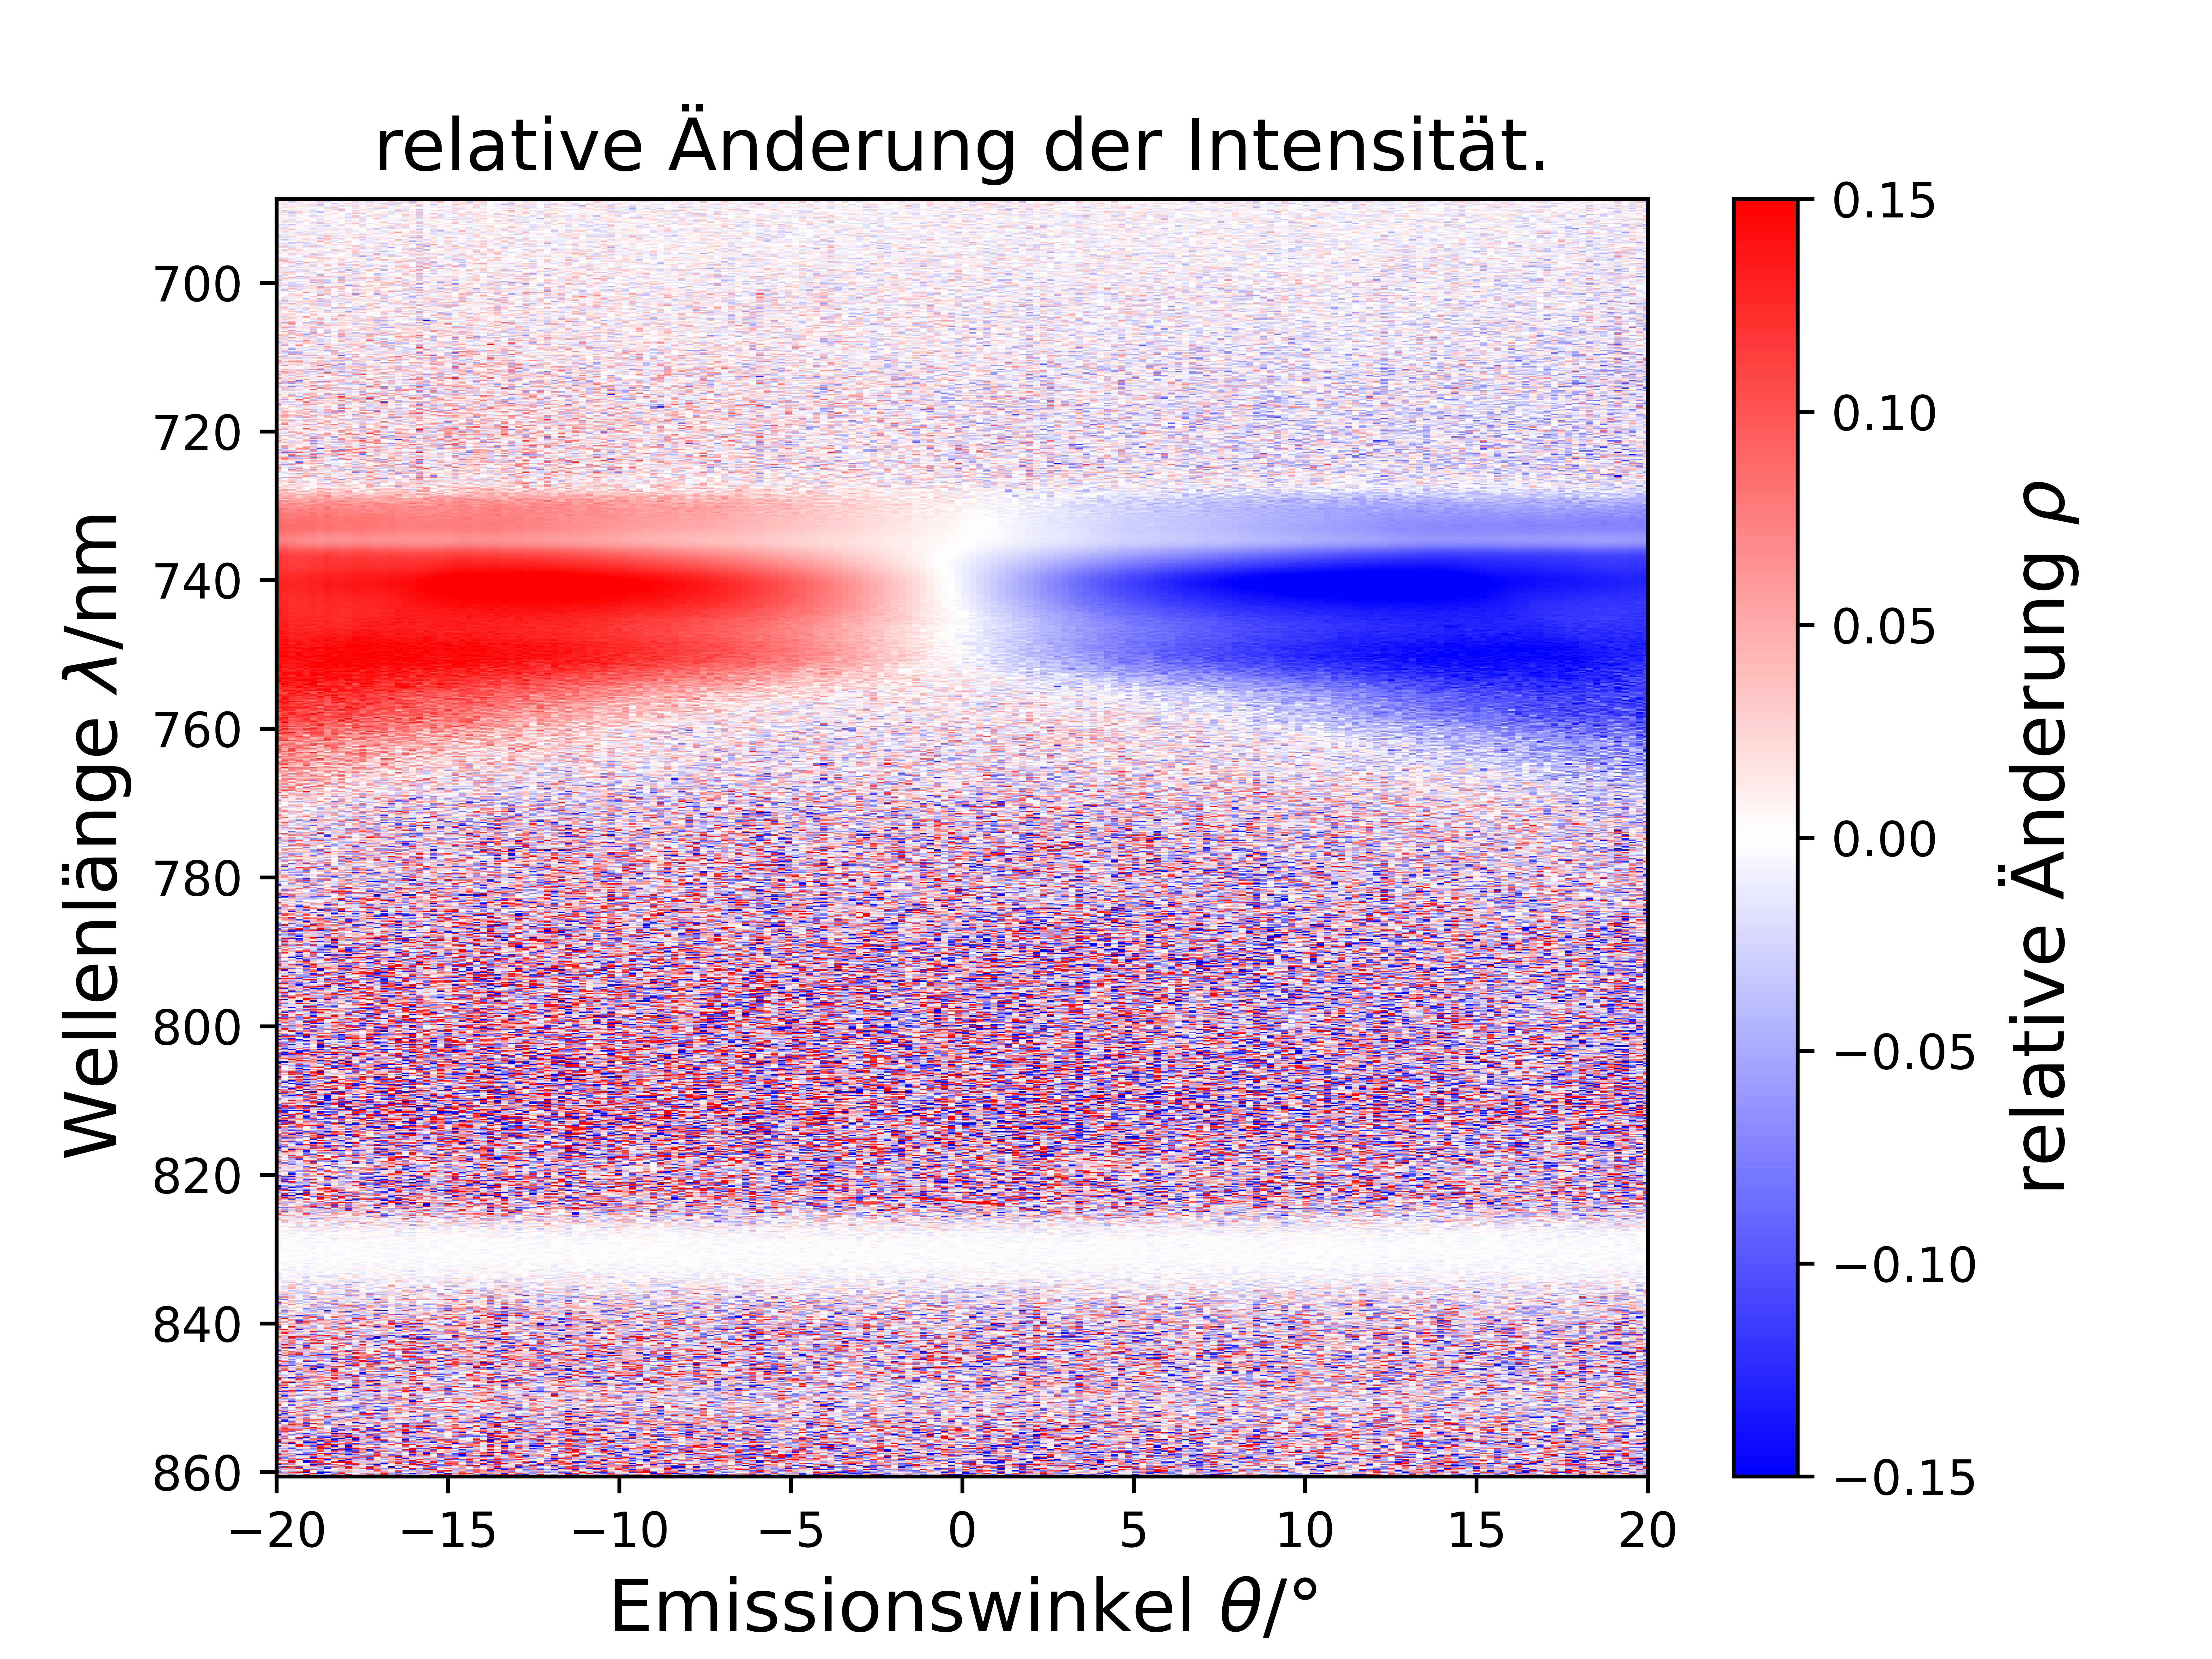
\includegraphics[scale=0.45]{./Plots/colormap_rel_change_intensity_022818A 250nm 4K 2020-07-14_komplett.png}
        \caption{Gemessene Direktionalität, des vollständigen\\ Sensors, bei einer Temperatur von $\SI{4}{\kelvin}$.}
        \label{fig:rel_komplett}
    \end{subfigure}
    \begin{subfigure}{0.50\textwidth}
        %\centering
        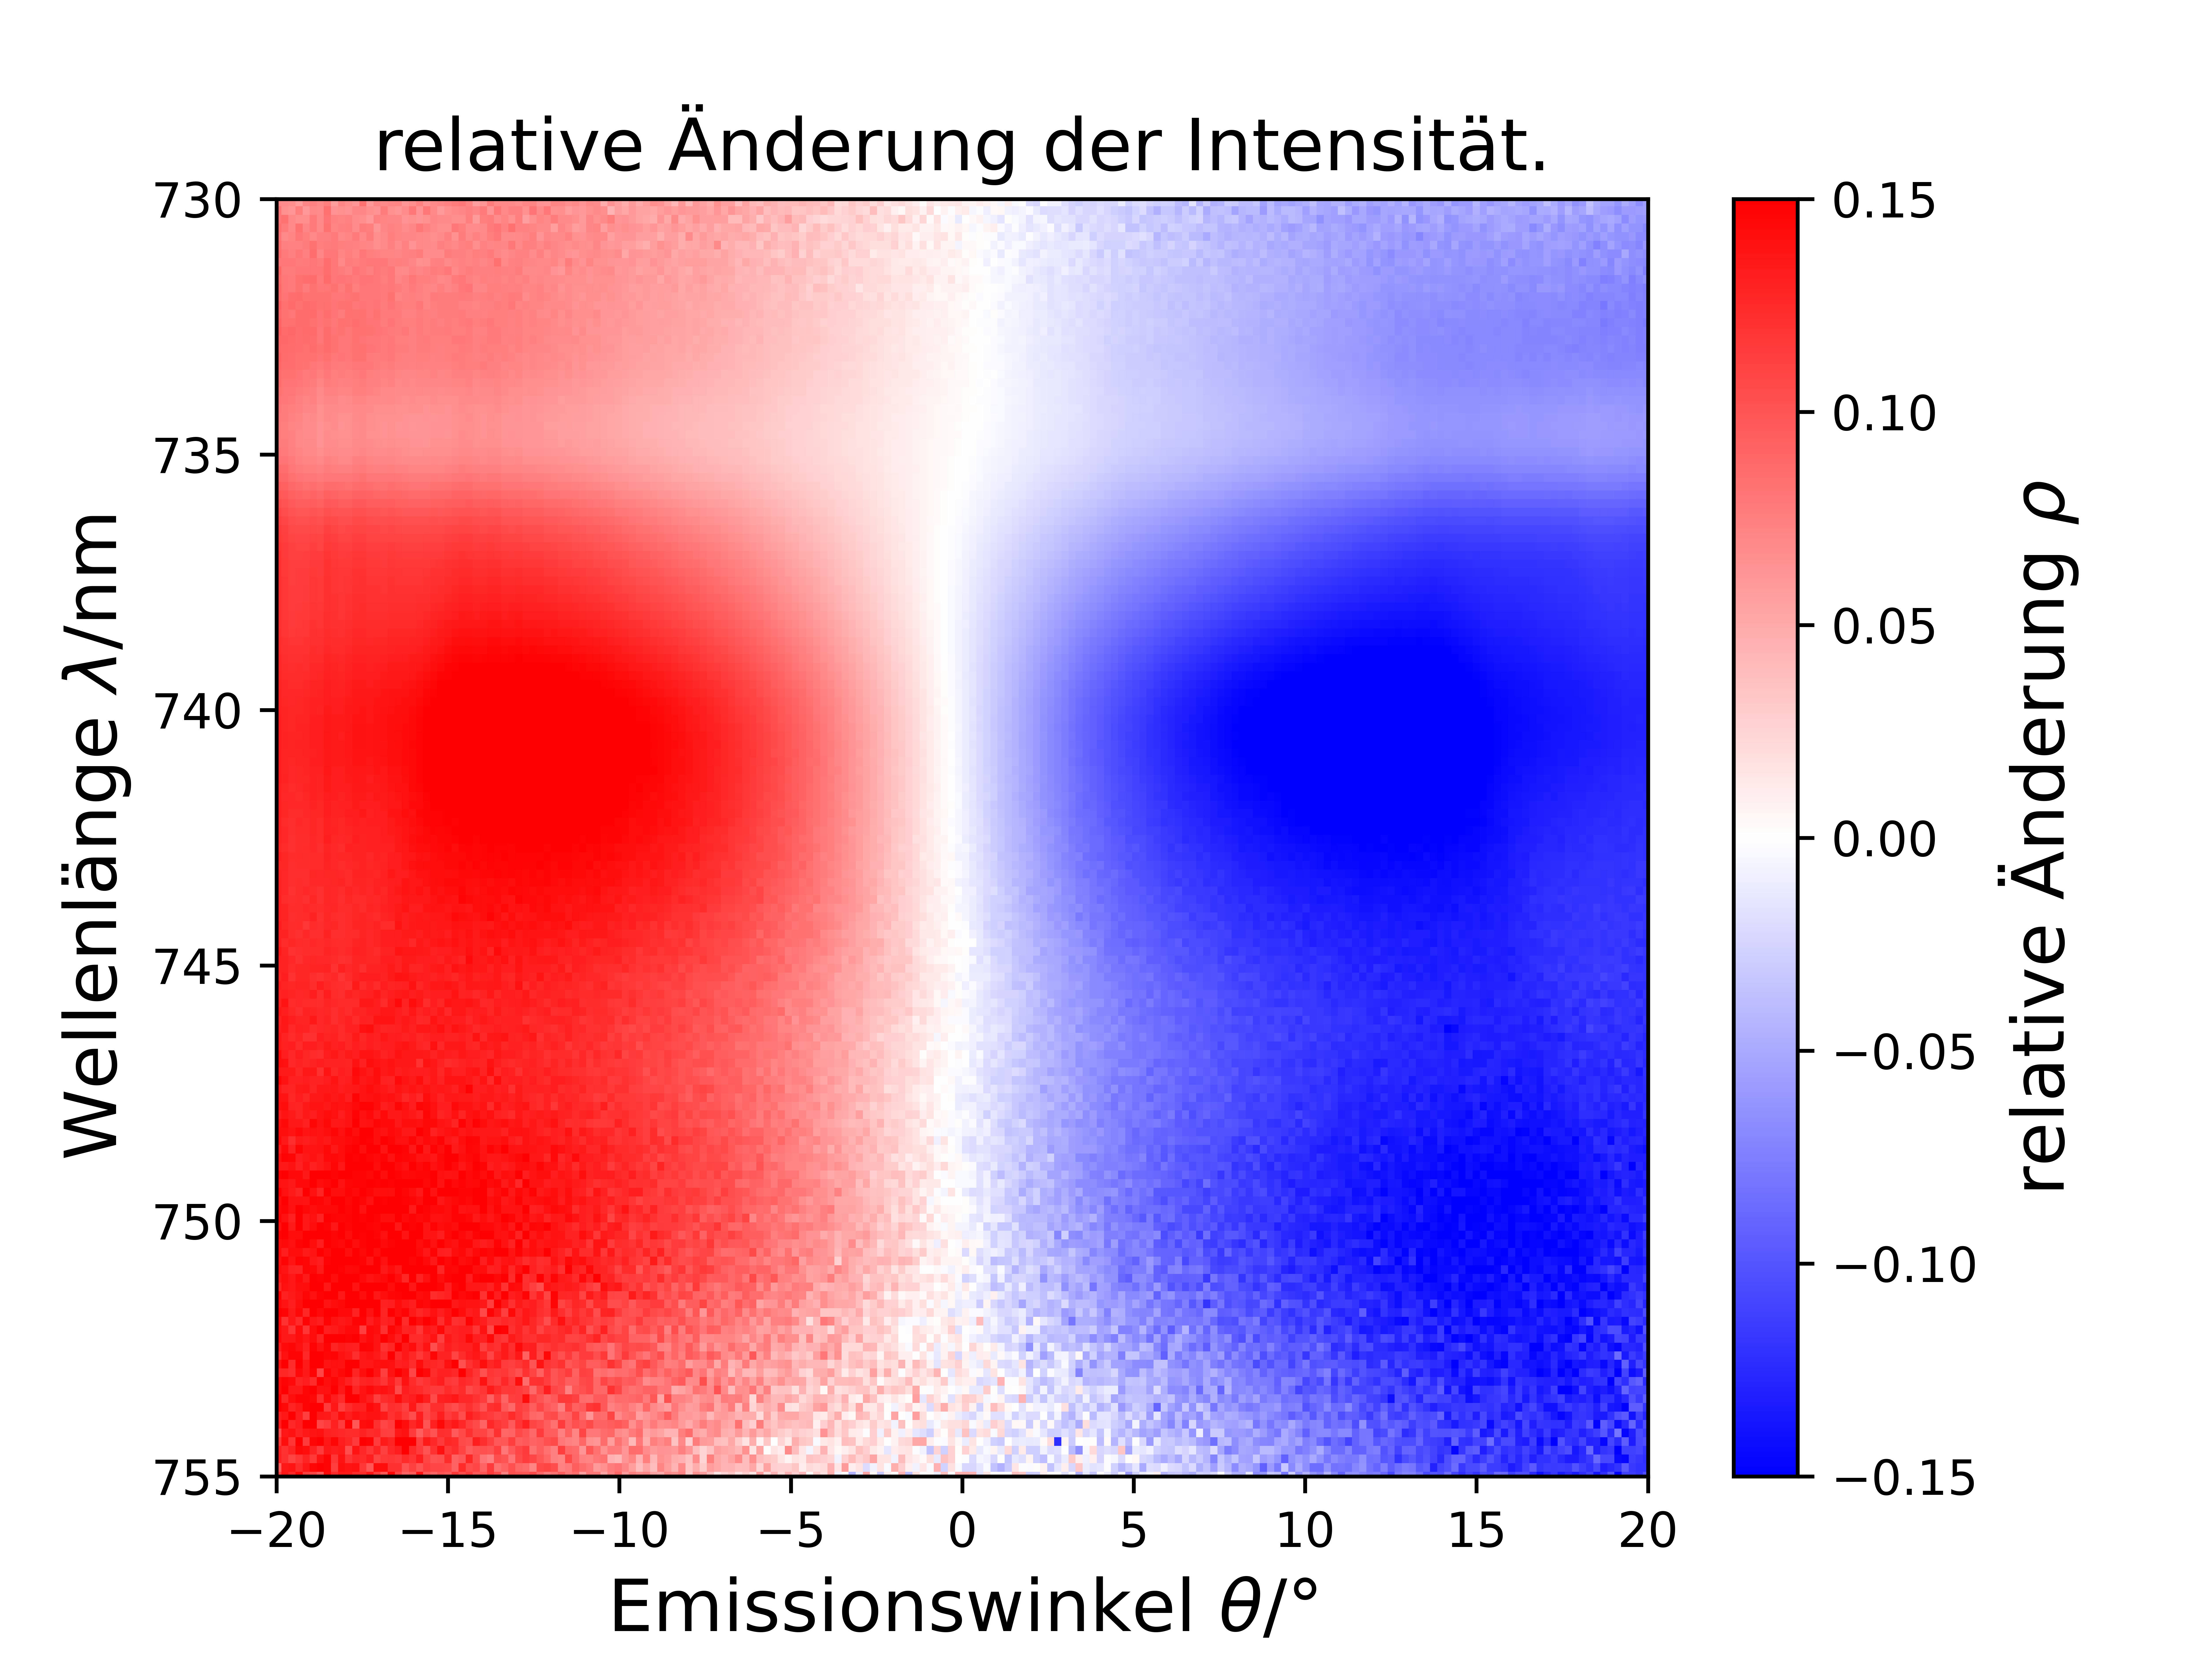
\includegraphics[scale=0.45]{./Plots/colormap_rel_change_intensity_022818A 250nm 4K 2020-07-14.png}
        \caption{Gemessene Direktionalität im Bereich von $\SI{730}{\nano\meter}$ bis $\SI{755}{\nano\meter}$
        bei einer Temperatur von $\SI{4}{\kelvin}$.}
        \label{fig:rel}
    \end{subfigure}
    \caption{Darstellung der Direktionalität in verschiedenen Wellenlängenbereichen.}
    \label{fig:rho}
\end{figure}
\FloatBarrier

Die Direktionalität $\rho$ berechnet sich durch 
\begin{equation}
    \rho = \frac{I_\text{B+} - I_\text{B-} }{ I_\text{B+} + I_\text{B-} }.
\end{equation}
Dabei ist $I_\text{B+}$ die Intensität bei positiven Magnetfeld und $I_\text{B-}$ bei negativen Magnetfeld.
Die Direktionalität in Prozent gibt an, wie sehr sich die Lichtemission in eine Richtung bei Umpolung des Magnetfelds ändert. 
Der Maximalwert von $\rho$ beträgt somit $1$.
%Eine farbliche Darstellung ist in Abbildung~\ref{fig:rel_komplett}zu sehen. %Doppelt?
Der maximal gemessene Wert der Direktionalität im Experiment beträgt $\pm \SI{15}{\percent}$. 
Das bedeutet konkret, dass das ausgesendete Licht der Probe, die PL, $\SI{15}{\percent}$ stärker in eine Richtung
emittiert wird, wenn das Magnetfeld eine bestimmte Polung besitzt.
Der weisse Balken der im Wellenlängenbereich von ca. $\SI{825}{\nano\meter}$ bis $\SI{835}{\nano\meter}$ 
in Abbildung\ref{fig:rel_komplett} zu sehen ist, 
hat seinen Ursprung im verwendten Substrat GaAs. Da dieses ebenfalls zum Leucheten angeregt wird.
GaAs hat allerdings keine magnetischen Eigenschaften, darum entfällt die Beeinflussung durch das angelegte Magnetfeld
und es ist keine Direktionalität erkennbar.
 % GaAs strahlt aber wie und warum ? da es nicht magnetisch ist 
%kann ist es unempfunlich gegeb das magnetfelg ==> kein effekt
Der Restbereich, d.h. der Bereich ohne Signifikanten Effekt, besteht aus einem statistischen Pixelrauschen der CCD.

In Abbildung~\ref{fig:rel} ist der reine Bereich der Direktionalität dargestellt.
Hier ist ebenfalls eine weisse Linie (vertikal) in der Mitte des Graphen bei $\theta = \SI{0}{\degree}$ zu erkennen.
Dieser Bereich entsteht da bei einem Winkel von $\theta = \SI{0}{\degree}$ das PL genau senkrecht aus der Probe kommt
und somit keine Direktionalität aufweisen kann.
Die schwächere horizontale Linie bei $\lambda = \SI{735}{\nano\meter}$ 
(vgl. Abbildung~\ref{fig:rho}) entsteht durch 
ausgesendetes Licht der Probe welches sich mit dem eigentlichen Effekt überlagert. 
Es wird vermutet das dieses Licht aus den Randbereichen der Probe und/oder aus den Zwischenbereichen des Goldgitters 
emittiert wird.

Die Direktionalität im Maximum der Photolumineszenz (bei $\lambda = \SI{737}{\nano\meter}$) beträgt
$\rho = \SI{11,5}{\percent}$. 
Dieser Verlauf der Direktionalität bei konstanter Wellenlänge ist in Abbildung~\ref{fig:dir} dargestellt.
\begin{figure}
    \centering
    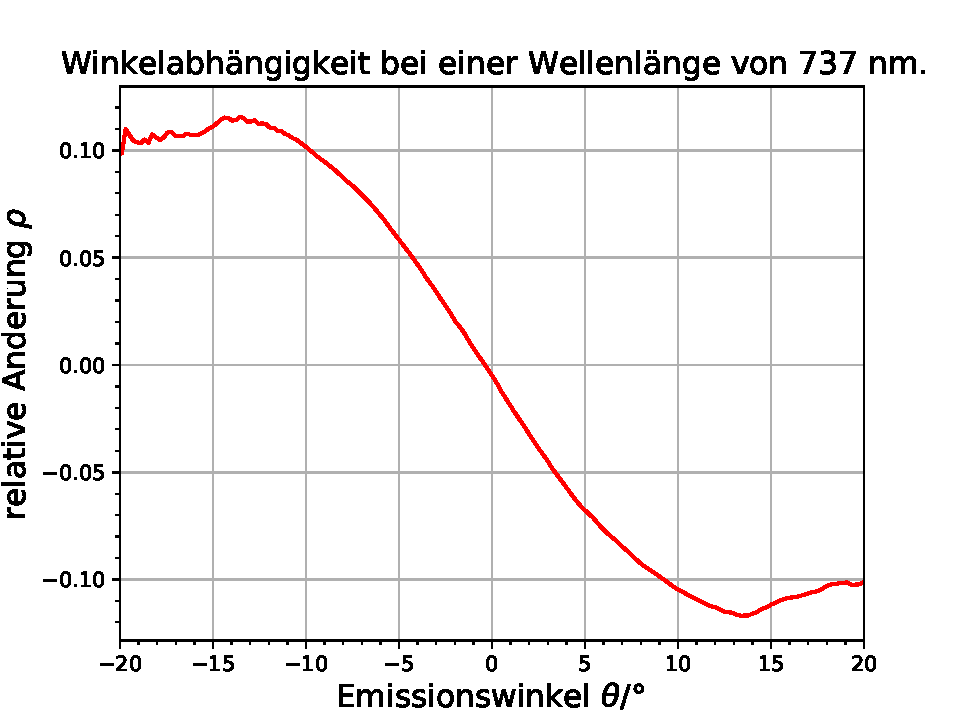
\includegraphics[scale=0.7]{./Plots/rho_at_specific_wavelength_737_nm_022818A 250nm 4K 2020-07-14.pdf}
    \caption{Gemessene Direktionalität $\rho$ im Maximum der Photolumineszenz.
    Der Wert der im Experiment gemessen Direktionalität ist $\rho = \SI{11,5}{\percent}$.}
    \label{fig:dir}
\end{figure}
\FloatBarrier

Der Graph von $\rho$ ist bis auf eine kleine Abweichung am Nullpunkt (vgl. Abbildung~\ref{fig:dir}) 
Antisymmetrisch. 
Das Ergebnis der Antisymmetrie deckt sich ist wie bereits oben genannt mit der Theorie, denn das einzige was eine
Änderung des Magnetfelds bewirkt ist ein Vorzeichenwechsel der Direktionalität.
Bei genauerer Betrachtung des Graphen der Direktionalität lässt sich erkennen, dass bis ca. $\theta = \pm \SI{5}{\degree}$
die Steigung von $\rho$ linear.
Wird dieser Wert über- bzw. unterschritten geht der Graph in eine Krümmung über die bei $\theta = \pm \SI{13,5}{\degree}$
ihr Maximum besitzt. 
Hinter dem Maximum schwächt sich die Direktionalität ab.
Da bereits in mehreren Experimenten unabhängig dieser Arbeit bestätigt wird, dass der Graph
der Direktionalität Antisymmetrisch ist, wird die Abweichung um $\theta = \SI{0}{\degree}$
korrigiert.
Dazu wird der Direktionalitätsfaktor $c_0$ eingeführt. 

Der Graph von $\rho$ lässt sich mit der Gleichung 
\begin{equation}
    c_0= \frac{\rho(-\theta)-\rho(\theta)}{2}
    \label{eq:c_0} 
\end{equation}

um den Nullpunkt korrigieren, sodass er perfekt achsensymmetrisch ist.
Dies ist in Abbildung~\ref{fig:dir_kor} zu sehen.
\begin{figure}
    \centering
    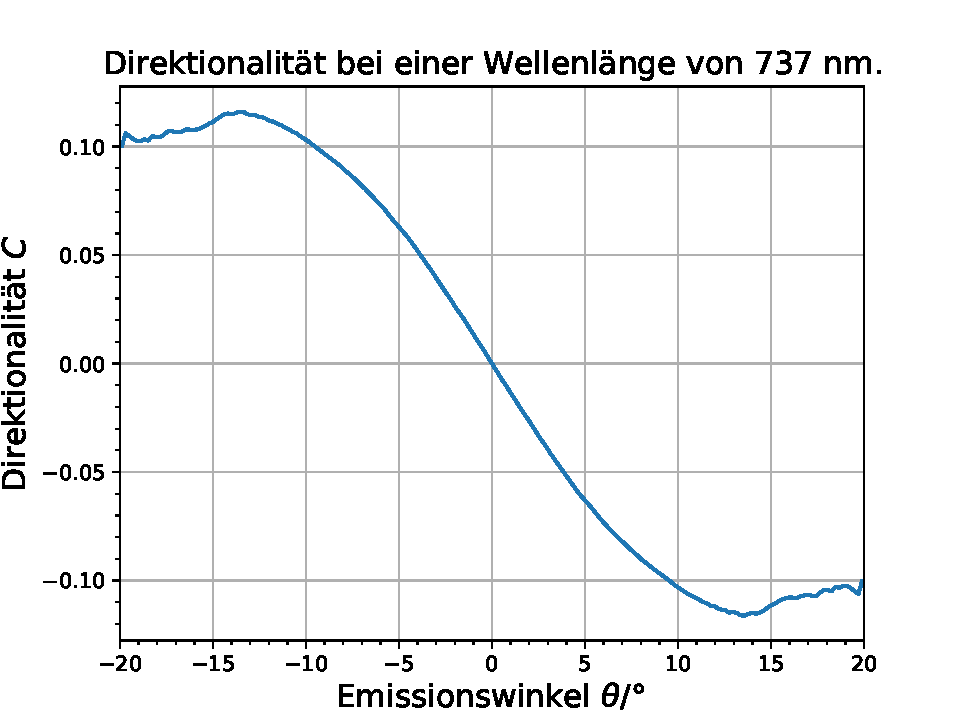
\includegraphics[scale=0.7]{./Plots/rho_at_specific_wavelength_737_nm_022818A 250nm 4K 2020-07-14_korrigiert.pdf}
    \caption{Gemessene um den Nullpunkt korrigierte Direktionalität $c_0$ im Maximum der Photolumineszenz.
    Der Wert der im Experiment gemessen Direktionalität ist $\rho = \SI{11,5}{\percent}$.}
    \label{fig:dir_kor}
\end{figure}
\FloatBarrier


\section{Temperatur Abhängigkeit der Direktionalität}
Im folgenden Abschnitt der Arbeit wird die Temperaturabhängigkeit der im Experiment
beobachteten Direktionalität diskutiert und wesentliche Aspekte erläutert.

Die Probe wurde über einem Temperaturbereich von $ \Delta T =\SI{41}{\kelvin} $ gemessen.
Die kleinste eingestellte Temperatur ist dabei $T =\SI{4}{\kelvin}$ gewesen, die größte 
$T =\SI{45}{\kelvin}$.
Es sind insgesamt 11 Temperaturabhängige Messungen entstanden.

Die Wellenlänge bei der alle nachfolgenden Graphen betrachtet werden ist $\lambda =\SI{738}{\nano\meter}$ 
(vgl. Abbildung~\ref{fig:temp_all_nach}), da sich das gemittelte Maximum der Photolumineszenz bei
$\lambda =\SI{737,7}{\nano\meter}$ befindet.
Im Abbildung~\ref{fig:int_temp} sind die Intensitätsmaxima bei den unterschiedlichen Temperaturen zu sehen.
Klar erkennbar ist hier ebenfalls der Verlauf einer Gaußschen Glockenfunktion.
\begin{figure}
    \centering
    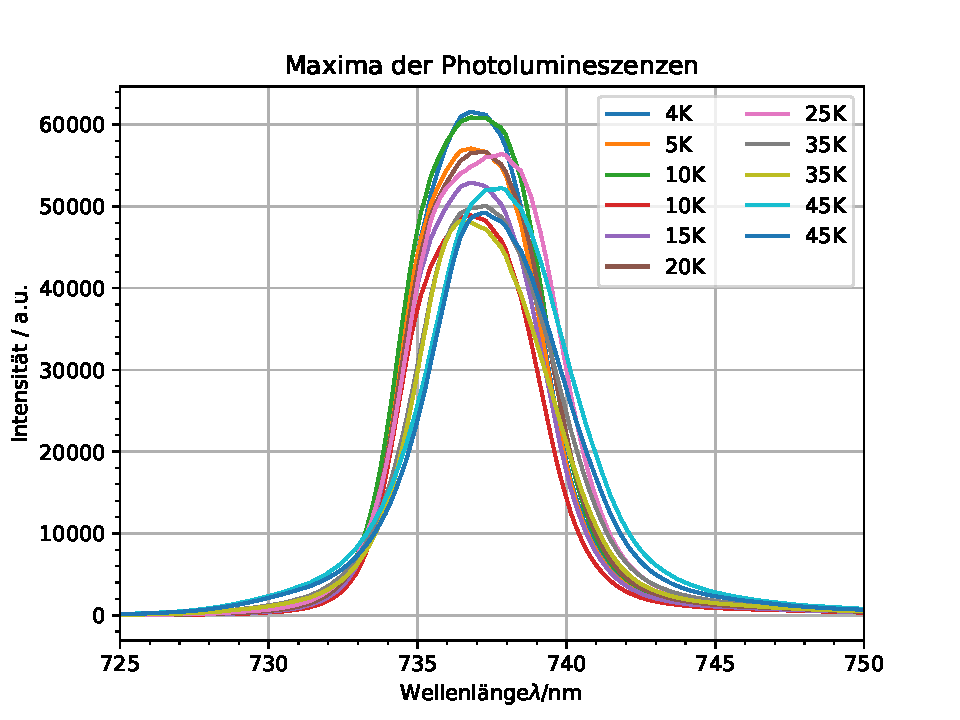
\includegraphics[scale=0.7]{./Plots/max_value_Pl_alle.pdf}
    \caption{Darstellung der Intensitätsmaxima bei unterschiedlichen Temperaturen.
    Das gemittelte Maxima ist bei $\lambda =\SI{737,7}{\nano\meter}$.}
    \label{fig:int_temp}
\end{figure}
\FloatBarrier 

In Abbildung~\ref{fig:temp_all_nach} sind die unterschiedlichen Verläufe
aller ermittelten Direktionalitäten, bei konstanter Wellenlänge, abgebildet.
%\begin{figure}
%    \centering
%    \begin{subfigure}{0.55\textwidth}
%       %\centering
%        \includegraphics[scale=0.45]{./Plots/Temperaturabhaengigkeit_rho_at_738_nm_4K5K10K10K15K20K25K35K35K45K45K_vorher.pdf}
%        \caption{Darstellung der Direktionalität $\rho$ bei konstanter Wellenlänge und  unterschiedlichen Temperaturen.
%         Die Wellenlänge beträgt $\lambda =\SI{738}{\nano\meter}$.}
%        \label{fig:temp_all_vor}
%    \end{subfigure}
%    \begin{subfigure}{0.55\textwidth}
%        %\centering
%        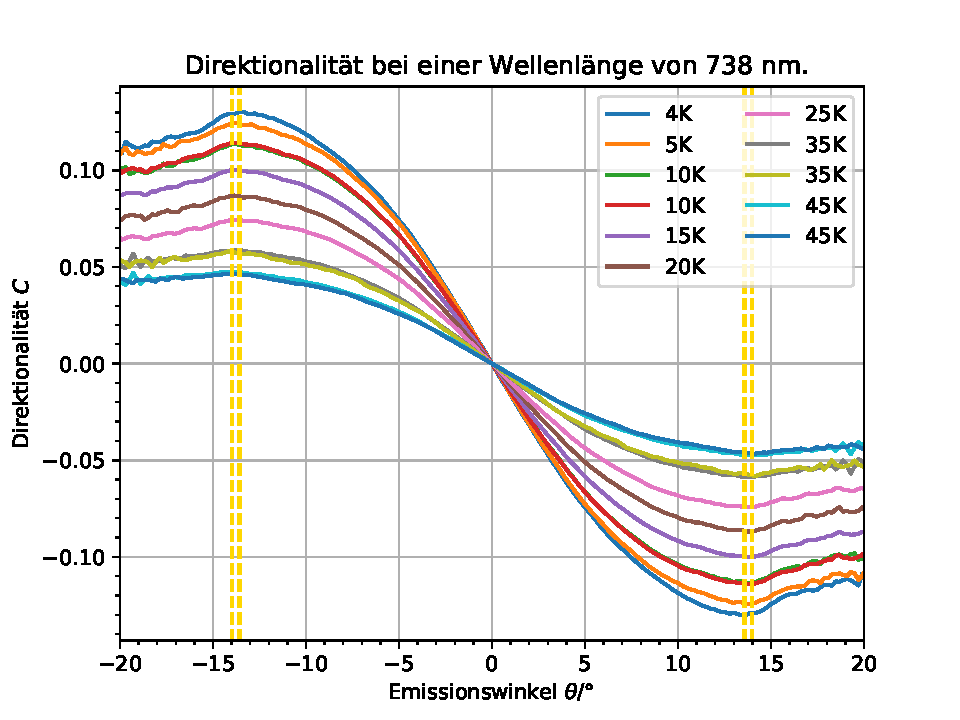
\includegraphics[scale=0.45]{./Plots/Temperaturabhaengigkeit_rho_at_738_nm_4K5K10K10K15K20K25K35K35K45K45K_korrigiert.pdf}
%        \caption{Darstellung der Direktionalität $c_0$ bei konstanter Wellenlänge und  unterschiedlichen Temperaturen.
%         Die Wellenlänge beträgt $\lambda =\SI{738}{\nano\meter}$.}
%        \label{fig:temp_all_nach}
%    \end{subfigure}
%    \caption{In der linken Abbildung ist die Direktionalität $\rho$ zu sehen, in der rechten der Direktionalitätsfaktor $c_0$.}
%    \label{fig:temp_verlauf}
%\end{figure}
%\FloatBarrier
%TODO fix der zeichnungen
\begin{figure}
    \centering
    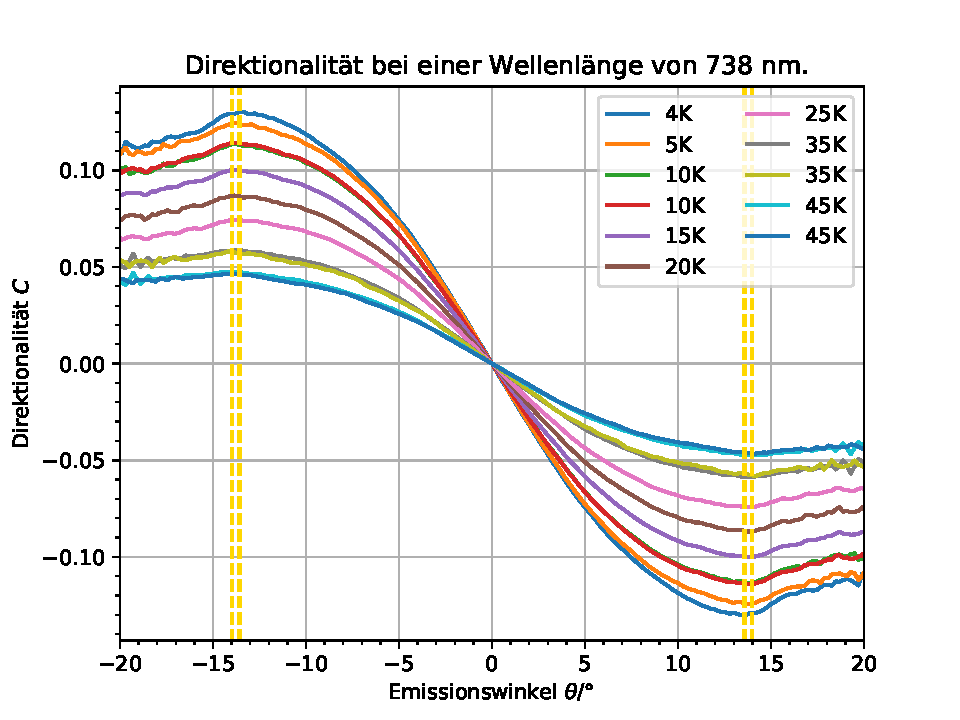
\includegraphics[scale=0.7]{./Plots/Temperaturabhaengigkeit_rho_at_738_nm_4K5K10K10K15K20K25K35K35K45K45K_korrigiert.pdf}
    \caption{Darstellung des Direktionalitätsfaktors $c_0$ bei konstanter Wellenlänge und  unterschiedlichen Temperaturen.
    Die Wellenlänge beträgt $\lambda =\SI{738}{\nano\meter}$.}
    \label{fig:temp_all_nach}
\end{figure}
\FloatBarrier

Die gelb gestrichelten Linien in Abbildung~\ref{fig:temp_all_nach} markieren die Bereiche 
in denen die Maxima der Direktionalitäten\footnote{Im weiteren Verlauf wird
von Direktionalität gesprochen auch wenn $c_0$ statt $\rho$ dargestellt ist.} 
bei den unterschiedlichen Temperaturen liegen.
Der Winkelbereich in denen sich die Maxima befinden erstreckt sich von  $\theta = \pm \SI{13,58}{\degree} 
$ bis $ \theta = \pm \SI{13,98}{\degree}$.
%In Tabelle~\ref{tab:rc} ist ein Vergleich der Werte von $\rho$ und $c_0$ zu dargestellt.  
Bei Betrachtung der Graphen mit gleicher Temperatur (z.B. $\SI{10}{\kelvin}$) 
überlappt sich die Funktion von $c_0$ sehr gut.
Bei unterschiedlichen Temperaturen lässt sich ein deutlicher Unterschied erkennen.
Graphisch entsteht eine sichtbare Abflachung und Erniedrigung des Verlaufs von $c_0$.
Das bedeutet konkret, dass der Effekt der Direktionalität mit der Temperatur sinkt.
Sehr deutlich ist das bei Betrachtung der beiden Randwerte 
der Temperaturen $T = \SI{4}{\kelvin}$ und $ T = \SI{45}{\kelvin}$ zu sehen.
Die Direktionalität fällt hier von $c_0= \SI{13.04}{\percent}$ auf $c_0 = \SI{4,77}{\percent}$ ab.

Werden die jeweiligen Maximalwerte der Direktionalität $c_0$ in Abhängigkeit
der Temperatur gepottet entsteht der Graph in Abbildung~\ref{fig:fit}


maximum korrgegtur
dann 4stuckrausgenimen bvild 